\scanpage{5}
\mspage{3}
\margin{\figure{\begin{tikzpicture}\draw (0,0)--(.6,-.65);\end{tikzpicture}}}

\figure{
\begin{tikzpicture}[baseline=(t.base)]\node (t) {3};\draw (0,0) ellipse (0.23 and 0.28);\end{tikzpicture}}
\uline{pg23}\quad On peut dire plus simplement que ${}_nK$ est étale séparé car ${}_nK=\operatorname{Ker}({}_nG\longrightarrow{}_nH)$. En a), ne dirais-tu pas que ${}_nK_{\bar s}$ est isomorphe à un sous-groupe de ${}_nK_{\bar t}$.

\uline{pg24}\quad a) $\ell\,15$ :\quad
\figure{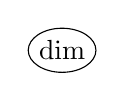
\begin{tikzpicture}[baseline=(t.base)]\node[inner sep=2pt] (t) {$\dim$};\draw (0,0) ellipse (0.43 and 0.28);\end{tikzpicture}}
$\operatorname{Ker}(u_{\unsure{\eta|s}})=0$\quad ?

\figure{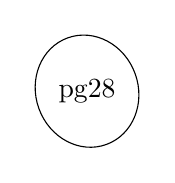
\begin{tikzpicture}[baseline=(t.base)]\node[inner sep=3pt] (t) {\uline{pg28}};\draw[rotate=20] (0,0) ellipse (0.65 and 0.72);\end{tikzpicture}}
Les notions introduites dans 3.5 ont elles été définies pour $S$ non hensélien ? (il faudrait au moins choisir un groupe d'inertie).
\inserted{[itou pour 3.7]}

\uline{pg29}\quad $\ell-2$\quad la terminologie ``clôture normale'' est-elle encore canonique ?

\figure{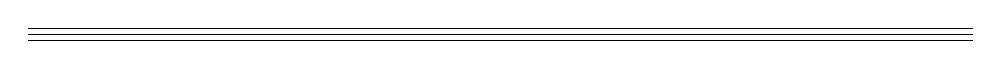
\begin{tikzpicture}\draw (0,0)--(12,0);\draw (0,-0.08)--(12,-0.08);\draw (0,-0.16)--(12,-0.16);\end{tikzpicture}}

\figure{
\begin{tikzpicture}[baseline=(t.base)]\node (t) {4};\draw (0,0) ellipse (0.22 and 0.26);\end{tikzpicture}}
\uline{p32}\quad $\ell\,8$\quad ne dépend
\figure{
\begin{tikzpicture}[baseline=(t.base)]\node[inner sep=2pt] (t) {pas};\draw (0,0) ellipse (0.28 and 0.27);\end{tikzpicture}}

\figure{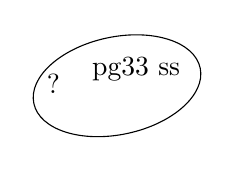
\begin{tikzpicture}[baseline=(t.base)]\node[inner sep=3pt] (t) {\uline{pg33 ss}};\node at (-1.05,-0.18) {?};\draw[rotate=12] (-0.28,-0.15) ellipse (1.08 and 0.62);\end{tikzpicture}}
(4.2)\quad Ne donnerais tu pas un énoncé style ``voisinage tubulaire'' compréhensible. La vérité est

\deleted{\unsure{a)}} on a un morphisme de topos $\operatorname{Spec}(K)_{\mathrm{et}}\xrightarrow{\varphi}\operatorname{Spec}(k)_{\mathrm{et}}$ (``\unsure{ext.|ent.} du corps résiduel'') et $A_0^0$ est un schéma relatif sur $(\operatorname{Spec}(\unsure{k|K}))_{\mathrm{et}}$ annelé par $\varphi^*\mathcal O$ [le $\varphi^*$ des faisceaux d'ensembles]. Même chose d'ailleurs pour
\figure{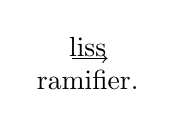
\begin{tikzpicture}[baseline=(t.base)]\node (t) at (0,0) {\unsure{liss}};\draw[->] (-0.2,-0.15)--(0.25,-0.15);\node at (0,-0.42) {\unsure{ramifier}.};\end{tikzpicture}}
$A_0$

\figure{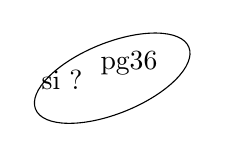
\begin{tikzpicture}[baseline=(t.base)]\node[inner sep=3pt] (t) {\uline{pg36}};\node at (-0.85,-0.22) {\unsure{si} ?};\draw[rotate=22] (-0.27,-0.10) ellipse (1.05 and 0.45);\end{tikzpicture}}
$\ell-6$.\quad ``ce n'est pas la trace qui est \unsure{contragrédiente}; l'énoncé primitif était correct.

\uline{pg40}\quad (4.5.4)\quad Qu'est-il écrit dans la marge ?

$\ell-1$\quad Quel est loc cit. ?

$\ell\,3$\quad $\ell$-groupe signifie-t-il tué par $\ell$, ou par un $\ell^{\unsure{n}}$ ?

Le trait est-il strictement local ? ce serait plus agréable.

\margin{4}
